\documentclass[10pt]{beamer}
\usepackage{xeCJK}
\usepackage{graphicx}
\usepackage{booktabs}
\usepackage{listings}
\usepackage{multirow}
\usepackage{mathtools}
\usepackage{ulem}
\usefonttheme[onlymath]{serif}
\usetheme{metropolis}
\begin{document}
	\title{Water Problem Choose Talk}
	\date{\today}
	\maketitle
	\clearpage
	\begin{frame}{Invisiable Integers}

		invisible integers是一种简单的游戏,玩家通过一些提示来猜一个由数字$1$到$9$组成的隐藏序列。每一个提示都是一个由下列规则生成的由互不相同的数字组成的序列:

		从隐藏序列中选出任意的起始位置。

		选择一个方向---向左或者向右。

		从选择的起始位置开始、以选定的方向遍历隐藏序列中的整数,将没有出现在提示中的数加在提示末尾。

		找出一个最短的长度,使得存在一个在这个长度下满足所有提示的序列。

		提示个数不大于$10$。
	\end{frame}
	\clearpage
	\begin{frame}{Solution}
	
		\onslide<1-> 首先有一种简单的$O(n!\operatorname{poly}(n))$的做法:

		\onslide<2-> 考虑枚举每个提示向左$L$或向右$R$,枚举出现的顺序。

		\onslide<3-> 枚举$R_1$的起始位置,有用的信息只有$L_{1\dots x}$处理完了,$L_x$处理到了第$y$位。

		\onslide<4-> 发现继续枚举即可,不过需要想想怎么维护和继承信息。
	\end{frame}
	\clearpage
	\begin{frame}{维护}

		\onslide<1-> 考虑到向左的:
	
		$$
		\begin{aligned}
		\rm{\color{red}123}45\xrightarrow{2}&{\color{red}12}345\\
		\rm{\color{red}123}45\xrightarrow{4}&{\color{red}1234}5\\
		\rm{\color{red}123}45\xrightarrow{5}&{\color{red}123}45\\
		\rm{\color{red}123}45\xrightarrow{6}&-1\\
		\end{aligned}
		$$
		\onslide<2-> 考虑到向右的:
	
		$$
		\begin{aligned}
		\rm{\color{red}123}45\xrightarrow{2}&{\color{red}123}45\\
		\rm{\color{red}123}45\xrightarrow{4}&{\color{red}1234}5\\
		\rm{\color{red}123}45\xrightarrow{5}&-1\\
		\rm{\color{red}123}45\xrightarrow{6}&-1\\
		\end{aligned}
		$$
	
	\end{frame}
	\clearpage
	\begin{frame}
		\frametitle{继承}

		\onslide<1-> 向左的相当于依次插入。

		\onslide<2-> 向右的有些麻烦,如果12345,在处理完12后,可以在后面接一个1345的。
		
		\onslide<3-> 即是在没处理完的时候继承。
	\end{frame}
	\clearpage
	\begin{frame}{整理一下}
	
		\onslide<1-> 维护信息比较简单,但是继承需要分两种:

		\begin{itemize}
			\item 向左的: 处理完$i$后,下一个是$j$,$j$的信息就是空的依次加上$i$的元素。
			\item 向右的: 处理$i$时,如果$i$依次加上$j$的元素后是整个$i$,那么可以视为处理完了$i$,然后从$j$的开头处理$j$。
		\end{itemize}
	
	\end{frame}
	\clearpage
	\begin{frame}{回到那个暴力}
	
		\onslide<1-> 可以DP,记当前DP到了$i,j,k,l$,即当前处理的向左的是$i$,处理了$j$位,向右的是$k$,处理了$l$位。

		\onslide<2-> 复杂度:$O(n!9^5)=O(n!)$?
	
	\end{frame}
	\clearpage
	\begin{frame}{solution}
	
		\onslide<1-> 考虑到这是不是可以状压。

		\onslide<2-> 有用的状态只有那个$i,j,k,l$,和每个位置是否被处理过。

		\onslide<3-> 于是就可以直接优化了,有亿点细节,复杂度$O(2^n\operatorname{poly}(n))$。
	\end{frame}
	\clearpage
	\begin{frame}{Gomoku}
	
		这是一道交互题。

		五子棋是一种两个人在二维棋盘上玩的游戏。棋盘上的每个格子可以为空,放有第一名玩家的棋子(黑),或者放有第二名玩家的棋子(白),但是不能都有。初始时所有的格子都是空的。两个玩家轮流操作,从第一名玩家开始。每次操作,一名玩家可以把他的棋子放进恰好一个空格子里。首先在一行中放下五个相邻棋子的玩家获胜。一行可以是横行、竖行或对角线。

		在这个问题中,玩家们使用 $19\times 19$ 的棋盘。如果整个棋盘都放满了棋子但无人获胜,游戏平局。
	\end{frame}
	\clearpage

	\begin{frame}{Gomoku}
		第一名玩家将会使用下面的策略:第一次操作时,她会把她的棋子放到棋盘的正中间。在后面的每次操作中,她会选择一个下子后局面分数最大的位置下子。

		为了计算一个局面的分数,第一名玩家会考虑能组成胜利组合的所有地方——换句话说,棋盘上所有横行、竖行、对角线上五个连续的格子(当然,它们会互相重叠)。如果这一行同时包括了第一名玩家的棋子和第二名玩家的棋子,就无视它。如果这一行包括了恰好 $k (1\le k\le 5)$ 个第一名玩家的棋子而没有第二名玩家的棋子,给该局面的分数加上 $50^{2k−1}$。如果这一行包括了恰好 $k$ 个第二名玩家的棋子而没有第一名玩家的棋子,给该局面的分数减去 $50^{2k}$。最后,给分数加上一个 $0$ 到 $50^2−1$ 的随机数。随机数是均匀分布的。

		如果第一名玩家有多个分数相同的格子可选(因为上面提到的随机分数的原因,这是非常罕见的),第一名玩家选择 X 坐标最小的位置,如果仍有多个格子有相同的 X 坐标,就选择 Y 坐标最小的位置。

		你的任务是,写一个程序扮演第二名玩家,并打败上述的策略。
	\end{frame}
	\clearpage
	\begin{frame}{solution}
	
		如图(按字母顺序下):

		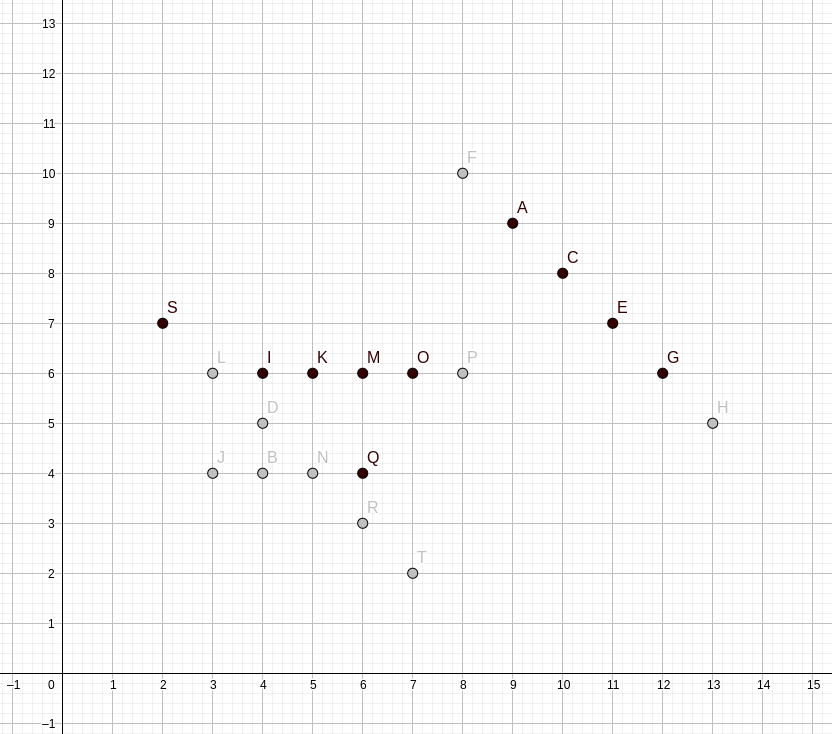
\includegraphics[width=0.8\textwidth]{1.png}

	
	\end{frame}
\end{document}